\documentclass[tikz,border=6pt]{standalone}
\usepackage{tikz}
\usetikzlibrary{arrows.meta, positioning, fit, backgrounds, calc}
\begin{document}
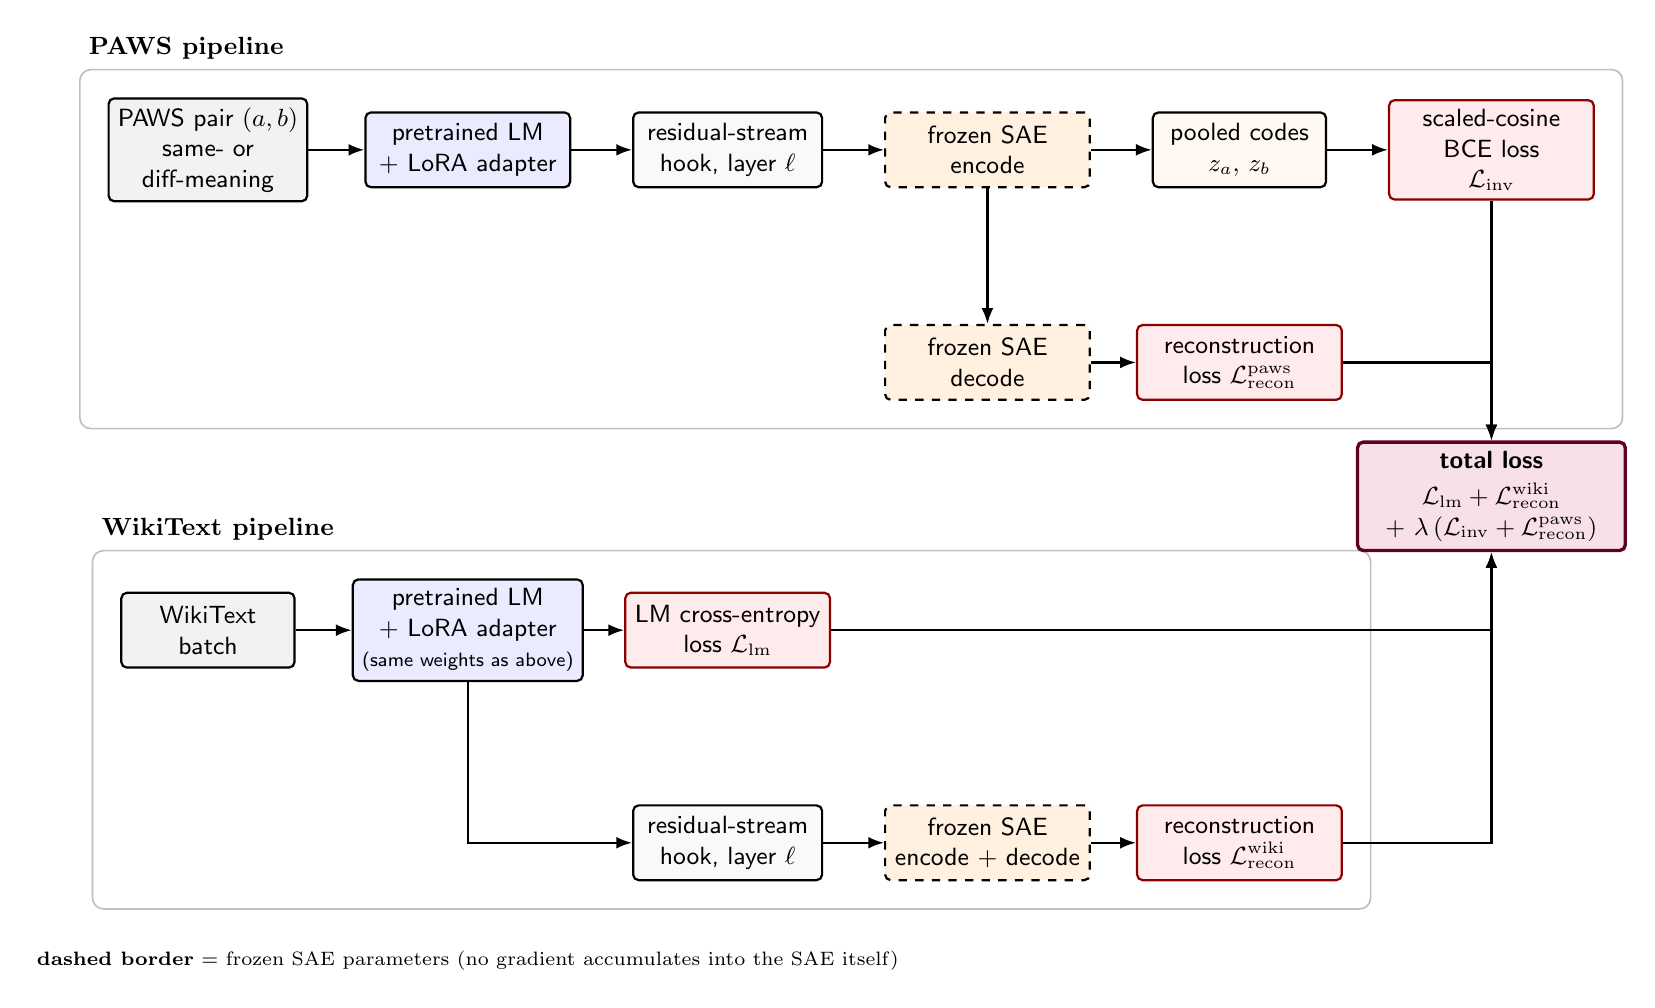
\begin{tikzpicture}[
    font=\sffamily\small,
    box/.style={draw, rounded corners=2pt, minimum height=0.95cm, align=center, line width=0.8pt, minimum width=2.6cm},
    inputbox/.style={box, fill=gray!10, minimum width=2.2cm},
    lmbox/.style={box, fill=blue!8},
    saebox/.style={box, fill=orange!12, dashed},
    lossbox/.style={box, fill=red!8, draw=red!55!black},
    totalbox/.style={box, fill=purple!12, draw=purple!50!black, minimum width=3.4cm, minimum height=1.3cm, line width=1.2pt},
    arrow/.style={-{Latex[length=2mm]}, line width=0.8pt},
    panel/.style={draw=black!25, rounded corners=4pt, line width=0.6pt, inner sep=10pt},
]

% ===================== PANEL A: PAWS pipeline (top) =====================
\node[inputbox] (paws) at (0,8.3) {PAWS pair $(a,b)$\\ same- or\\ diff-meaning};
\node[lmbox] (lm1) at (3.3,8.3) {pretrained LM\\ + LoRA adapter};
\node[box, fill=gray!5, minimum width=2.4cm] (hook1) at (6.6,8.3) {residual-stream\\ hook, layer $\ell$};
\node[saebox] (sae1) at (9.9,8.3) {frozen SAE\\ encode};
\node[box, fill=orange!5, minimum width=2.2cm] (pool1) at (13.1,8.3) {pooled codes\\ $z_a,\,z_b$};
\node[lossbox] (lbce) at (16.3,8.3) {scaled-cosine\\ BCE loss\\ $\mathcal{L}_{\mathrm{inv}}$};

\draw[arrow] (paws) -- (lm1);
\draw[arrow] (lm1) -- (hook1);
\draw[arrow] (hook1) -- (sae1);
\draw[arrow] (sae1) -- (pool1);
\draw[arrow] (pool1) -- (lbce);

\node[saebox] (sae1d) at (9.9,5.6) {frozen SAE\\ decode};
\node[lossbox] (lrecp) at (13.1,5.6) {reconstruction\\ loss $\mathcal{L}_{\mathrm{recon}}^{\mathrm{paws}}$};
\draw[arrow] (sae1) -- (sae1d);
\draw[arrow] (sae1d) -- (lrecp);

\begin{scope}[on background layer]
\node[panel, fit=(paws)(lm1)(hook1)(sae1)(pool1)(lbce)(sae1d)(lrecp)] (panelA) {};
\end{scope}
\node[font=\bfseries\small, anchor=south west] at (panelA.north west) {PAWS pipeline};

% ===================== PANEL B: WikiText pipeline (bottom) =====================
\node[inputbox] (wiki) at (0,2.2) {WikiText\\ batch};
\node[lmbox] (lm2) at (3.3,2.2) {pretrained LM\\ + LoRA adapter\\ \scriptsize(same weights as above)};
\node[lossbox] (llm) at (6.6,2.2) {LM cross-entropy\\ loss $\mathcal{L}_{\mathrm{lm}}$};

\draw[arrow] (wiki) -- (lm2);
\draw[arrow] (lm2) -- (llm);

\node[box, fill=gray!5, minimum width=2.4cm] (hook2) at (6.6,-0.5) {residual-stream\\ hook, layer $\ell$};
\node[saebox] (sae2) at (9.9,-0.5) {frozen SAE\\ encode + decode};
\node[lossbox] (lreconw) at (13.1,-0.5) {reconstruction\\ loss $\mathcal{L}_{\mathrm{recon}}^{\mathrm{wiki}}$};

\draw[arrow] (lm2) |- (hook2);
\draw[arrow] (hook2) -- (sae2);
\draw[arrow] (sae2) -- (lreconw);

\begin{scope}[on background layer]
\node[panel, fit=(wiki)(lm2)(hook2)(sae2)(lreconw)(llm)] (panelB) {};
\end{scope}
\node[font=\bfseries\small, anchor=south west] at (panelB.north west) {WikiText pipeline};

% ===================== Total loss =====================
\node[totalbox] (total) at (16.3,3.9) {\textbf{total loss}\\[2pt] $\mathcal{L}_{\mathrm{lm}} + \mathcal{L}_{\mathrm{recon}}^{\mathrm{wiki}}$\\ $+\ \lambda \left( \mathcal{L}_{\mathrm{inv}} + \mathcal{L}_{\mathrm{recon}}^{\mathrm{paws}} \right)$};

\draw[arrow] (lbce.south) -- (total.north);
\draw[arrow] (lrecp.east) -| (total.north);
\draw[arrow] (lreconw.east) -| (total.south);
\draw[arrow] (llm.east) -| (total.south);

% gradient path back
% \draw[arrow, blue!55!black, line width=1.1pt, dash pattern=on 4pt off 2pt]
%   (total.north) to[out=110,in=0] (17.5,10.8) to[out=180,in=90] (3.3,9.9) -- (lm1.north);
% \node[align=center, font=\scriptsize, blue!55!black] at (10.4,11.1) {gradient flows back only into the LoRA parameters of the shared LM+LoRA (both panels use the same weights)};

\node[align=left, font=\scriptsize] at (3.3,-2.0) {\textbf{dashed border} = frozen SAE parameters (no gradient accumulates into the SAE itself)};

\end{tikzpicture}
\end{document}
